\subsection{Processo di sviluppo}
\label{subsection:processo_sviluppo}
ll processo di sviluppo riguarda l'insieme di attività necessarie per produrre e implementare il software, assicurandosi che risponda ai requisiti definiti e sia di qualità adeguata.

\subsubsection{Analisi dei requisiti}
\label{subsubsection:analisi_requisiti}
L'analisi dei requisiti è una attività cruciale nel \glossario{ciclo di vita} del software, in cui vengono raccolte, analizzate e documentate le esigenze degli \glossario{stakeholder} per definire chiaramente cosa il sistema dovrà fare. 
Questa attività produce il documento di analisi dei requisiti descritto nella sezione \hyperref[subsec:documentazione]{Documentazione}.

\paragraph{Requisiti}
I requisiti vengono esaminati a due livelli di astrazione differenti e quindi categorizzati in due macro categorie:
\begin{enumerate}
    \item \textbf{Requisiti utente}: descrivono le esigenze degli \glossario{stackeholder} dal punto di vista degli utenti del sistema.
    Questi requisiti vengono estrapolati dal capitolato, dagli incontri interni e dagli incontri con la proponente;

    \item \textbf{Requisiti software}: descrivono come le caratteristiche che il sistema dovrà avere per soddisfare i primi.
    Questi requisiti vengono ottenuti tramite l'analisi dei precedenti, quindi un singolo requisito utente viene soddisfatto da più \glossario{requisiti software}.
    Ogni \glossario{requisito software} può essere diviso in uno o più sotto requisiti che lo vanno a specificare.

\end{enumerate}
I requisiti di queste macro categorie possono poi essere categorizzati ulteriormente in:
\begin{enumerate}
    \item \textbf{Requisiti funzionali}
    
    Rappresentano ciò che un sistema deve fare per soddisfare le esigenze degli utenti o degli \glossario{stakeholders};

    \item \textbf{Requisiti qualitativi}
    
    I requisiti di qualità (requisiti non funzionali) descrivono caratteristiche qualitative del sistema, come prestazioni, sicurezza, usabilità e manutenibilità;

    \item \textbf{Di vincolo}
    
    I requisiti di vincolo (requisiti non funzionali) rappresentano limitazioni o condizioni obbligatorie che influenzano lo sviluppo, l'implementazione o l'operatività del sistema. 

\end{enumerate}
I \glossario{requisiti utente} vengono identificati usando lo schema:
\begin{lstlisting}
    RU[priorita]-[identificativo] 
\end{lstlisting}
Dove:
\begin{enumerate}
    \item \textbf{priorità}: \lstinline{O} per obbligatorio e \lstinline{F} per facoltativo;
    \item \textbf{identificativo}: numero univoco crescente.
\end{enumerate}
I \glossario{requisiti software} vengono identificati usando lo schema:
\begin{lstlisting}
    R[tipo][priorita]-[identificativo].[sotto requisito] 
\end{lstlisting}
Dove:
\begin{enumerate}
    \item \textbf{tipo}: \lstinline{F} per funzionale, \lstinline{Q} per qualità e \lstinline{V} per vincolo;
    \item \textbf{priorità}: \lstinline{O} per obbligatorio e \lstinline{F} per facoltativo;
    \item \textbf{identificativo}: numero crescente univoco all'interno del tipo del requisito.
    \item \textbf{sotto requisito}: numero crescente univoco all'interno dell'insieme dei sotto requisiti del requisito principale.
\end{enumerate}


\paragraph{Casi d'uso}
\label{par:casi_uso}
I casi d'uso forniscono una descrizione dettagliata delle funzionalità del sistema dal punto di vista degli utenti, delineando come il sistema deve rispondere a specifiche azioni o scenari. 
In particolare, un caso d'uso rappresenta un uso completo del sistema dalla prospettiva dell'utente.
I casi d'uso vengono rappresentati tramite una combinazione di descrizione e diagramma \glossario{UML} e sono usati per approfondire i \glossario{requisiti utente}.

\subparagraph{Descrizione}
Nella \hyperref[tab:template_casi_uso]{Tabella \ref{tab:template_casi_uso}} viene mostrato il template per la descrizione dei casi d'uso.
Ogni descrizione di caso d'uso deve includere:
\begin{enumerate}
    \item \textbf{Identificativo}: indicato usando lo schema \texttt{UC-<ID>}.
    Dove:
    \begin{enumerate}
        \item \texttt{<ID>}: identificativo numerico del caso d'uso (numero crescente).
    \end{enumerate}

    \item \textbf{Requisito utente}: requisito utente a cui fa riferimento il diagramma;

    \item \textbf{Pre-condizioni}: stato iniziale del sistema o vincoli necessari per l'attivazione del caso d'uso;

    \item \textbf{Post-condizioni}: stato finale del sistema dopo un esecuzione normale (priva di errori) del caso d'uso;

    \item \textbf{Attori}: entità esterna (\underline{umana o meno}) al sistema che interagisce con il software per iniziare o per contribuire al compimento dell'esecuzione di un caso d'uso.  
    Gli attori si dividono in:
    \begin{enumerate}
        \item  \textbf{Attori primari}: attori principali che partecipano al caso d'uso, solitamente contengono gli attori che iniziano l'interazione e/o sono i destinatari delle informazioni in output del caso d'uso;
        \item \textbf{Attore secondario}: altri attori coinvolti che non sono protagonisti nell'esecuzione del caso d'uso e non sono sotto il controllo diretto del sistema.
    \end{enumerate}

    \item \textbf{Trigger}: evento eseguito da un attore che attiva il caso d'uso;

    \item \textbf{Scenario principale}: sequenza di step che vengono portati a termine in un esecuzione normale del caso d'uso;
    
    \item \textbf{Scenari alternativi}: deviazioni o eccezioni rispetto allo scenario principale.
\end{enumerate}

\begin{usecase}{\texttt{<identificativo caso d'uso>}}{\texttt{<descrizione caso d'uso>}}
            
    \req{\texttt{<link requisito utente>}}
    
    \pre{
        \item \texttt{<pre condizione>}
        \item \texttt{<pre condizione>}
    }
    
    \post {
        \item \texttt{<post condizione>}
        \item \texttt{<post condizione>}
    }
    
    \actor{\texttt{<attore principale>}}
    
    \subactors{\texttt{<lista attori secondari>}}

    \trigger{\texttt{<trigger>}}
    
    \inc{\texttt{<lista casi d'uso inclusi>}}
    
    \base{\texttt{<caso d'uso di base>}}
    
    \scenario{
        \item \texttt{<$1^a$ azione>}
        \item \texttt{<$2^a$ azione>}
        \item \texttt{<<include:id>>}
    }

    \subscenario{
        \item[1.1] \texttt{<condizione branch dalla $1^a$ azione>}
        \begin{itemize}
            \item [a.] \texttt{$1^a$ azione del scenario secondario}
            \item [b.] \texttt{$2^a$ azione del scenario secondario}
        \end{itemize} 
        \item[2.1] \texttt{<condizione branch dalla $2^a$ azione>}
        \begin{itemize}
            \item [a.] \texttt{$1^a$ azione del scenario secondario}
            \item [b.] \texttt{$2^a$ azione del scenario secondario}
        \end{itemize} 
    }
    \caption{Template casi d'uso.}
    \label{tab:template_casi_uso}
\end{usecase}


\subparagraph{Diagrammi dei casi d'uso}
I diagrammi dei casi d'uso sono basati sul linguaggio \glossario{UML} (Unified Modeling Language), questi diagrammi illustrano i principali scenari operativi del sistema e aiutano a identificare e chiarire i \glossario{requisiti funzionali}.
Ogni diagramma è composto da:
\begin{itemize}
    \item \textbf{Sistema}: delimita i confini del sistema software, indicando quali funzionalità sono incluse e quali sono esterne a esso.
    Il sistema viene rappresentato nei diagrammi come mostrato in \hyperref[fig:sistema_uml]{Figura \ref{fig:sistema_uml}};
    \begin{figure}[H]
        \centering
        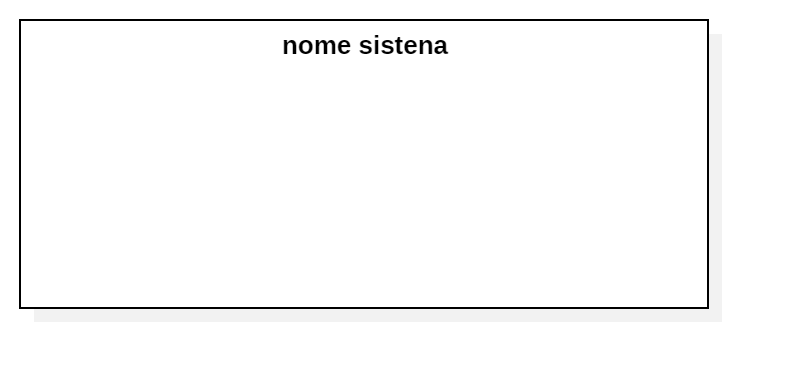
\includegraphics[scale=0.4]{Sezioni/ProcessiPrimari/Immagini/sistema.png}
        \caption{Rappresentazione del sistema in \glossario{UML}.}
        \label{fig:sistema_uml}
    \end{figure}
    
    \item \textbf{Attori}: rappresentano soggetti (persone, altri applicativi o dispositivi) esterni al sistema che vi interagiscono.
    Un attore viene rappresentato nei diagrammi usando la notazione mostrata in \hyperref[fig:attori_uml]{Figura \ref{fig:attori_uml}} e viene posta al di fuori del sistema;
    \begin{figure}[H]
        \centering
        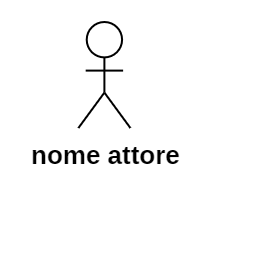
\includegraphics[scale=0.4]{Sezioni/ProcessiPrimari/Immagini/attori.png}
        \caption{Rappresentazione degli attori in \glossario{UML}.}
        \label{fig:attori_uml}
    \end{figure}
    
    \item \textbf{Casi d'uso}: rappresentano le funzionalità offerte dal sistema. 
    Ogni caso d'uso descrive una sequenza specifica di interazioni tra uno o più attori e il sistema.
    Ogni caso d'uso viene rappresentato nei diagrammi usando la notazione mostrata in \hyperref[fig:caso_uso]{Figura \ref{fig:caso_uso}};
    \begin{figure}[H]
        \centering
        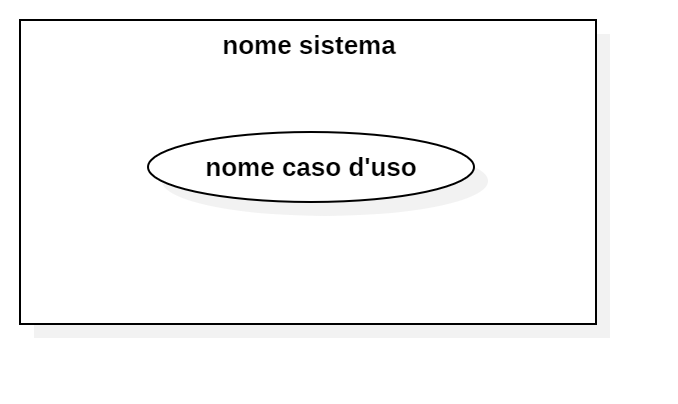
\includegraphics[scale=0.4]{Sezioni/ProcessiPrimari/Immagini/caso_uso.png}
        \caption{Rappresentazione caso d'uso in \glossario{UML}.}
        \label{fig:caso_uso}
    \end{figure}
    
    \item \textbf{Relazioni}: notazioni che permettono di rendere più modulari i diagrammi di casi d'uso e di rendere chiara l'interazione degli attori con il sistema.
    
    \begin{itemize}
        \item \textbf{Associazione}: è la relazione fondamentale che collega un attore a un caso d'uso a cui esso partecipa.
        Uno stesso attore può partecipare a un numero arbitrario di casi d'uso.
        Le associazioni vengono rappresentate in \glossario{UML} come mostrato in \hyperref[fig:associazione_uml]{Figura \ref{fig:associazione_uml}};
        \begin{figure}[H]
            \centering
            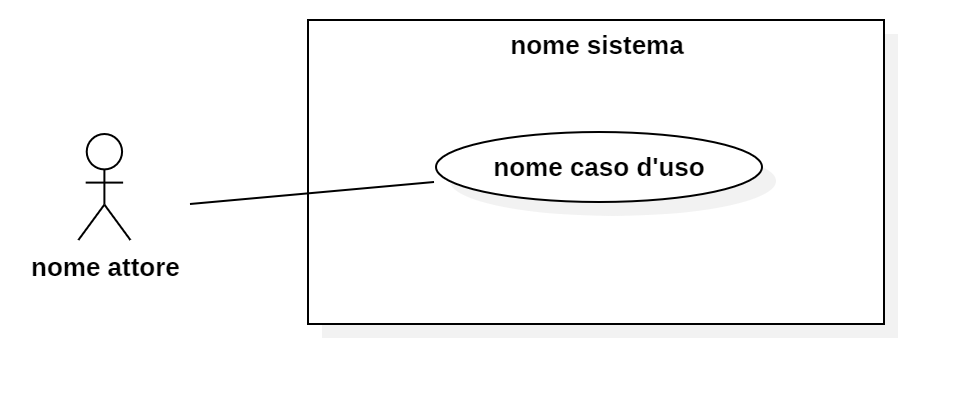
\includegraphics[scale=0.3]{Sezioni/ProcessiPrimari/Immagini/associazione.png}
            \caption{Rappresentazione associazione in \glossario{UML}.}
            \label{fig:associazione_uml}
        \end{figure}

        \item \textbf{Inclusione}: rappresenta una dipendenza in cui il comportamento del caso d'uso incluso è incorporato ogni volta che viene eseguito il caso d'uso base. 
        Il caso d'uso incluso non modifica le post condizioni del caso d'uso che lo include e quindi deve collaborare per raggiungere un obiettivo comune.
        L'inclusione viene rappresentata in \glossario{UML} come mostrato in \hyperref[fig:inclusione_uml]{Figura \ref{fig:inclusione_uml}};
        \begin{figure}[H]
            \centering
            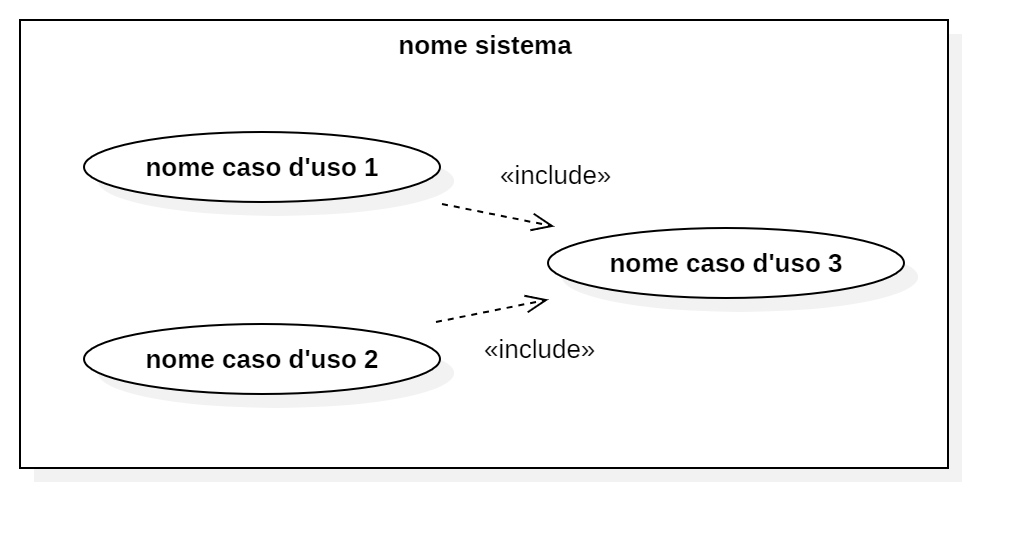
\includegraphics[scale=0.3]{Sezioni/ProcessiPrimari/Immagini/inclusione.png}
            \caption{Rappresentazione inclusione in \glossario{UML}.}
            \label{fig:inclusione_uml}
        \end{figure}

        \item \textbf{Estensione}: mostra una relazione in cui un caso d'uso esteso aumenta le funzionalità del caso d'uso principale e quindi modificando le post condizioni dello stesso. 
        Il caso d'uso esteso viene eseguito solo sotto determinate condizioni, interrompendo l'esecuzione del caso d'uso principale.
        L'estensione viene rappresentata in \glossario{UML} come mostrato in \hyperref[fig:estensione_uml]{Figura \ref{fig:estensione_uml}};
        \begin{figure}[H]
            \centering
            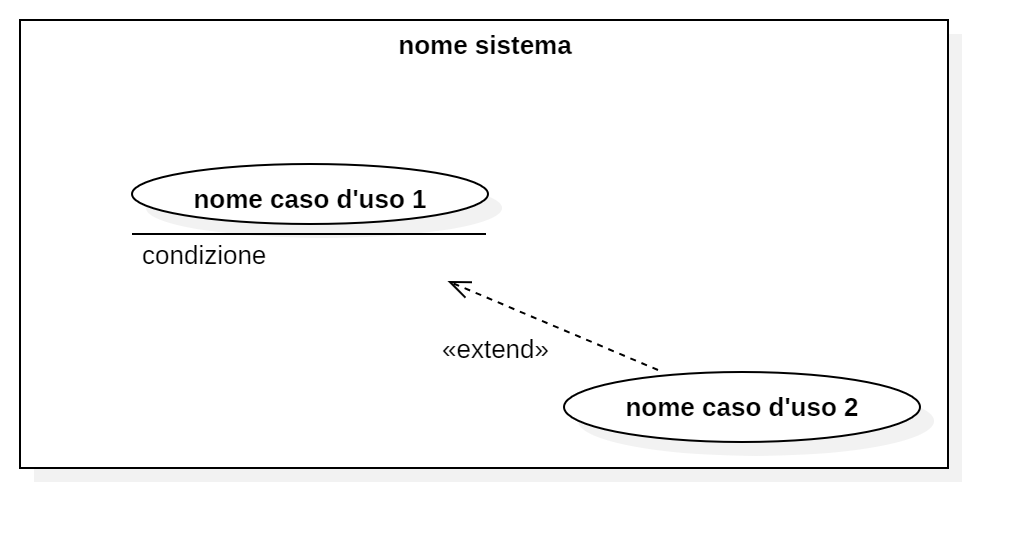
\includegraphics[scale=0.3]{Sezioni/ProcessiPrimari/Immagini/estensione.png}
            \caption{Rappresentazione estensione in \glossario{UML}.}
            \label{fig:estensione_uml}
        \end{figure}
        
        \item \textbf{Generalizzazione}: rappresenta una relazione in cui un caso d'uso figlio può aggiungere funzionalità o modificare il comportamento di un caso d'uso genitore. Tutte le funzionalità definite nel caso d'uso genitore si mantengono nel caso d'uso figlio se queste non vengono ridefinite.
        La generalizzazione viene rappresentata in \glossario{UML} come mostrato in \hyperref[fig:generalizzazione_uml]{Figura \ref{fig:generalizzazione_uml}};
        \begin{figure}[H]
            \centering
            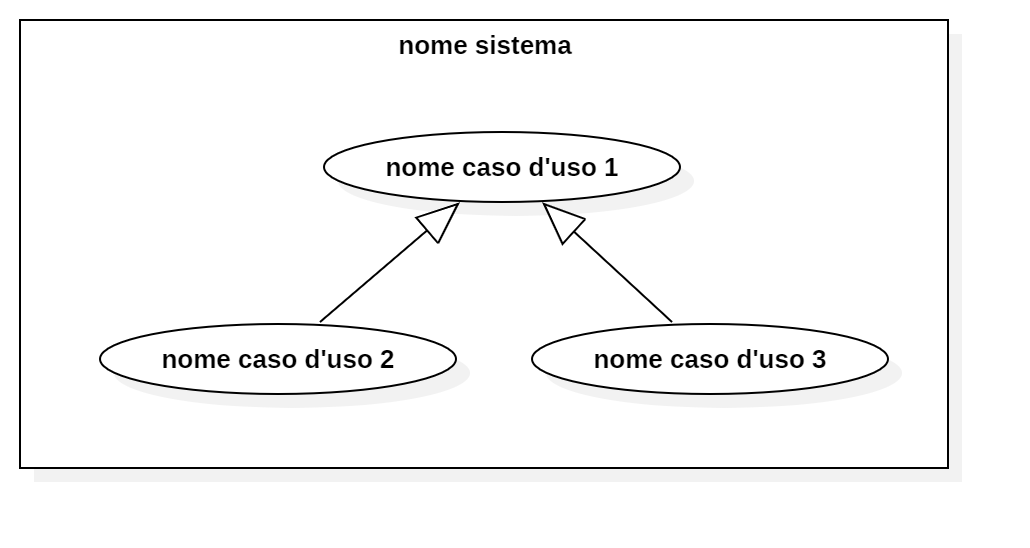
\includegraphics[scale=0.3]{Sezioni/ProcessiPrimari/Immagini/generalizzazione.png}
            \caption{Rappresentazione generalizzazione in \glossario{UML}.}
            \label{fig:generalizzazione_uml}
        \end{figure}
    \end{itemize}

    \item \textbf{Sottocasi d'uso}: i sottocasi d'uso rappresentano scenari specifici e dettagliati che si sviluppano all'interno di un caso d'uso principale. La loro funzione è di descrivere in modo approfondito le diverse situazioni o varianti operative che possono verificarsi nel contesto del caso d'uso generale.
\end{itemize}

\subsubsection{Progettazione}
\label{subsubsection:progettazione}
La progettazione è l'attività che definisce l'architettura del sistema software, fatta a seguito dell'attività di analisi, che descrive come il sistema soddisferà i requisiti definiti nel documento di \textit{Analisi dei Requisiti}.
L'attività di progettazione viene eseguita dal ruolo del progettista, tramite l'uso di pattern architetturali e di design, che permettono di definire la struttura e le relazioni tra le componenti del sistema.
Una buona progettazione deve garantire che l'architettura del sistema soddisfi i seguenti aspetti:
\begin{itemize}
    \item \textbf{Affidabilità}: deve garantire che il sistema funzioni nel modo previsto quando viene usato in condizioni previste;
    \item \textbf{Basso accoppiamento}: i moduli devono essere il meno possibile dipendenti tra loro;
    \item \textbf{Flessibilità}: deve avere la capacità di adattarsi a cambiamenti futuri;
    \item \textbf{Sufficienza}: l'architettura deve soddisfare tutti i requisiti definiti nell'analisi;
    \item \textbf{Efficienza}: garantisce un utilizzo efficiente delle risorse;
    \item \textbf{Incapsulamento}: i dettagli di implementazione di un modulo devono essere nascosti agli altri moduli;
    \item \textbf{Semplicità}: evita l'introduzione di elementi superflui;
    \item \textbf{Riusabilità}: deve essere possibile riutilizzare le parti dell'architettura in altri contesti;
    \item \textbf{Modularità}: suddivisione dell'architettura in moduli, in modo che le modifiche a uno di essi non influenzino gli altri;
    \item \textbf{Robustezza}: deve poter gestire situazioni di errore e di eccezione;
    \item \textbf{Coesione}: se esistono elementi che collaborano tra loro, devono essere raggruppati in un unico componente.
\end{itemize}

\paragraph{Fasi della progettazione}
La progettazione si suddivide in due fasi:
\begin{enumerate}
    \item \hyperref[subpar:progettazione_logica]{Progettazione logica};
    \item \hyperref[subpar:progettazione_dettaglio]{Progettazione di dettaglio}.
\end{enumerate}

\subparagraph{Progettazione logica}
\label{subpar:progettazione_logica}
La progettazione logica comprende la prima parte della progettazione del sistema, durante questa viene definita l'architettura del prodotto software.
Viene definita la struttura generale del sistema, i moduli principali e le relazioni tra di essi.
Per garantire la coerenza e la consistenza dell'architettura, il team andrà a usare stili architetturali che forniscono una soluzione progettuale di alto livello, guidando le scelte strutturali del sistema. 
Questo approccio assicura il soddisfacimento dei requisiti funzionali e non funzionali, come prestazioni, scalabilità e sicurezza, contribuendo alla manutenibilità e all'evoluzione del sistema nel tempo.
La fase di progettazione logica si suddivide in:
\begin{itemize}
    \item Individuazione delle componenti principali del sistema;
    \item Definizione delle interfacce e delle relazioni tra le componenti;
    \item Definizione delle strutture dati necessarie;
    \item Prima stesura del documento \textit{Manuale Utente};
    \item Stesura dei test di integrazione;
    \item Revisione delle soluzioni e dei pattern architetturali adottati.
\end{itemize}

\subparagraph{Istruzioni per la progettazione logica del front-end}
Per la progettazione logica delle componenti del front-end sono necessari:
\begin{itemize}
    \item \textbf{Descrizione}: descrizione delle funzionalità del componente;
    \item \textbf{Sotto componenti}: lista delle sotto componenti e loro funzione;
    \item \textbf{Tracciamento dei requisiti}: lista dei requisiti che vengono soddisfatti dalla componente.
\end{itemize}

\subparagraph{Istruzioni per la progettazione logica del back-end}
Per la progettazione logica delle componenti del back-end sono necessari:
\begin{itemize}
    \item \textbf{Descrizione}: descrizione delle funzionalità del componente;
    \item \textbf{Informazioni di route}: dettagli relativi alla configurazione e al comportamento delle route del componente;
    \item \textbf{Esecuzione}: descrizione dell'esecuzione della componente e dei suoi possibili output;
    \item \textbf{Tracciamento dei requisiti}: lista dei requisiti che vengono soddisfatti dalla componente.
\end{itemize}

\subparagraph{Progettazione di dettaglio}
\label{subpar:progettazione_dettaglio}
La progettazione di dettaglio è la seconda parte della progettazione del sistema, durante questa viene definita la struttura interna delle singole componenti individuate nella progettazione logica.
Ciò deve essere fatto prima della codifica del software, in modo da avere una visione chiara di come implementare le funzionalità richieste.
L'architettura deve essere tale da consentire a un singolo programmatore di poter codificare una singola unità architetturale.
Dunque ogni componente viene suddiviso in parti più piccole, le unità che a loro volta sono composte da moduli.
Lo scopo principale della progettazione di dettaglio è quello di organizzare la codifica del software, documentando le scelte di progettazione e collegando i requisiti a ogni singola unità.
Il sistema non deve essere però scomposto in unità troppo piccole, in quanto ciò potrebbe portare difficoltà nella coordinazione del lavoro del gruppo.
La fase di progettazione di dettaglio si suddivide in:
\begin{itemize}
    \item Descrizione dettagliata delle singole componenti, delle sue unità e dei moduli;
    \item Espansione e aggiornamento del documento \textit{Manuale Utente};
    \item Espansione e aggiornamento dei test di integrazione;
    \item Definizione dei test di unità;
\end{itemize} 

\subparagraph{Istruzioni per la progettazione di dettaglio del front-end}
Per la progettazione di dettaglio delle componenti del front-end sono necessari:
\begin{itemize}
    \item \textbf{Proprietà}: lista delle proprietà in input alla componente;
    \item \textbf{Eventi}: lista degli eventi in output dalla componente;
    \item \textbf{Aspetti principali}: lista degli aspetti principali della componente.
\end{itemize}

\subparagraph{Istruzioni per la progettazione di dettaglio del back-end}
Per la progettazione di dettaglio delle componenti del back-end sono necessari:
\begin{itemize}
    \item \textbf{Descrizione}: descrizione dettagliata della classe;
    \item \textbf{Diagramma della classe}: diagramma UML della classe;
    \item \textbf{Attributi}: lista (facoltativa) degli attributi della classe;
    \item \textbf{Operazioni}: lista (facoltativa) delle operazioni della classe;
    \item \textbf{Metodi}: lista (facoltativa) dei metodi della classe;
    \item \textbf{Implementazioni}: lista (facoltativa) delle interfacce implementate dalla classe;
    \item \textbf{Dipendenze}: lista (facoltativa) delle dipendenze della classe;
    \item \textbf{Estensioni}: lista (facoltativa) delle estensioni della classe.
\end{itemize}

\paragraph{Specifica Tecnica}
Diventa quindi essenziale documentare tramite il documento di \textit{Specifica Tecnica} l'intera fase di progettazione in modo chiaro e dettagliato, poiché sarà il punto di riferimento per la fase di codifica e di testing del software.
Il documento di \textit{Specifica Tecnica} va a trattare i seguenti argomenti:
\begin{itemize}
    \item \textbf{Tecnologie utilizzate}: descrizione delle tecnologie, dei framework e delle librerie utilizzate per lo sviluppo del software, motivando le scelte fatte;
    \item \textbf{Architettura generale}: descrizione dell'architettura generale del sistema e del \glossario{repository};
    \item \textbf{Progettazione logica}: descrizione delle funzionalità del sistema nel loro complesso, definendone le componenti principali ma non i dettagli;
    \item \textbf{Progettazione di dettaglio}: descrizione dettagliata e tecnica dell'implementazione dei moduli.
\end{itemize}


\paragraph{Strumenti}
Qui vengono elencati gli strumenti usati, che vengono poi approfonditi nella sezione \hyperref[sec:strumenti]{Strumenti}.
\begin{itemize}
    \item \glossario{LaTeX};
    \item \glossario{StarUML}.
\end{itemize}

\subsubsection{Testing del codice}
\label{subsubsec:testing_codice}
Il testing è una fase fondamentale del processo di sviluppo, volta a garantire la qualità e l'affidabilità del software, per questo motivo viene realizzata in parallelo all'attività di codifica.
Consiste nell'esecuzione di verifiche sistematiche per individuare errori, incongruenze e difformità rispetto ai requisiti. 
All'interno del progetto, il testing viene integrato nel flusso di sviluppo e include test automatizzati e manuali per assicurare la conformità del prodotto agli standard definiti.
Le categorie di testing eseguite precedentemente all'accettazione del software sono:
\begin{itemize}
    \item \textbf{Test di unità};
    \item \textbf{Test di integrazione};
    \item \textbf{Test di sistema};
\end{itemize}

\paragraph{Test di unità}
I test di unità sono una tipologia di test software che verificano il corretto funzionamento delle singole unità o componenti del codice, come funzioni, metodi o classi, in modo isolato. 
L'obiettivo principale è assicurarsi che ciascuna unità funzioni correttamente secondo le specifiche previste, facilitando l'individuazione precoce di eventuali errori o malfunzionamenti.
I test di unità vengono ideati durante la fase di progettazione di dettaglio per poi essere sviluppati in parallelo all'attività di codifica.
Per semplificare l'esecuzione dei test di unità vengono utilizzati i seguenti strumenti:
\begin{itemize}
    \item \textbf{Mock object}: oggetti configurabili che imitano il comportamento delle dipendenze reali (come Database o API), consentendo di verificare chiamate ai metodi e risposte attese;
    \item \textbf{Stub}: oggetti che restituiscono risposte predefinite per simulare il comportamento di dipendenze senza eseguire alcuna logica, usati per evitare chiamate reali a servizi esterni;
    \item \textbf{Driver}: moduli che simulano il comportamento di componenti chiamanti non ancora sviluppati.
\end{itemize}
Esistono tre tipi di tecniche di \textit{unit testing}:
\begin{itemize}
    \item \textbf{Black box testing}: questa tecnica di test viene utilizzata per coprire i test di unità relativi all'input, all'interfaccia utente e alle parti di output, senza considerare la struttura interna del codice;
    \item \textbf{White box testing}: questa tecnica verifica il comportamento funzionale del sistema fornendo input e controllando l'output, includendo l'analisi della struttura interna, del design e del codice dei moduli;
    \item \textbf{Grey box testing}: questa tecnica viene utilizzata per eseguire i casi di test, i metodi e le funzioni di test pertinenti, analizzando le prestazioni del codice nei moduli.
\end{itemize}
I test di unità vengono eseguiti in maniera automatizzata per garantire che ogni singola componente del software funzioni correttamente in modo isolato.
Questo viene fatto attraverso l'utilizzo di strumenti di automazione e framework specifici per i linguaggi di programmazione adottati durante lo sviluppo.

\paragraph{Test di integrazione}
I test di integrazione, o  sono una fase del processo di testing in cui si verificano le interazioni tra diverse unità o moduli del software, per assicurarsi che funzionino correttamente quando combinati. 
A differenza dei test di unità, che si concentrano su singole componenti isolando il loro comportamento, i test di integrazione verificano che i moduli collaborino come previsto, scambiandosi dati e interagendo senza problemi.
Questi test vengono definiti durante la progettazione ad alto livello e hanno lo scopo di rilevare difetti nell'architettura del software o una scarsa qualità dei test di unità.
Esistono due principali approcci all'\textit{integration testing}:
\begin{itemize}
    \item \textbf{Bottom-up}: in questo approccio, si parte testando i moduli di basso livello e si lavora verso l'alto, verificando prima i componenti più piccoli e fondamentali.
    In questo caso, si utilizzano \textit{driver} per simulare i moduli superiori non ancora implementati.
    Questo approccio è utile quando si vuole testare la stabilità delle basi del sistema prima di testare l'integrazione delle funzionalità più complesse;
    \item \textbf{Top-down}: in questo approccio, i test iniziano con i moduli di alto livello, quelli più vicini alla parte utente o alla logica di business del sistema.
    Le parti inferiori del sistema (come le dipendenze esterne o i moduli di basso livello) vengono simulate tramite \textit{stub}.
    Questo approccio è utile quando si vuole verificare l'integrazione delle funzionalità principali, prima di testare i dettagli più specifici.
\end{itemize}

\paragraph{Test di sistema}
I test di sistema sono una fase fondamentale del processo di testing in cui si verifica l'intero sistema software nel suo complesso, come una "black box".
Vengono eseguiti al completamento dei test di unità e di integrazione e hanno lo scopo di esaminare il software nel suo insieme, testando tutte le funzionalità e le interazioni tra i componenti per garantire che l'intero sistema funzioni come previsto.
Questi test includono la verifica dei requisiti funzionali e non funzionali del sistema definiti nel documento di \textit{Analisi dei Requisiti}, come la correttezza delle operazioni, le prestazioni e l'usabilità.
I test di sistema possono essere eseguiti in ambienti che simulano il contesto di produzione, assicurando che il sistema possa gestire il carico, le condizioni reali e che tutte le parti siano ben integrate.

\paragraph{Notazione dei test}
I test vengono indicati all'interno del documento \textit{Piano di Qualifica} e sono identificati così:
\begin{lstlisting}
    T.<Tipo>.<Numero>
\end{lstlisting} 
Dove:
\begin{itemize}
    \item \textbf{T}: indica la parola "test";
    \item \textbf{Tipo}: indica la tipologia del test, che può essere:
    \begin{itemize}
        \item \textbf{U}: test di unità;
        \item \textbf{I}: test di integrazione;
        \item \textbf{S}: test di sistema;
        \item \textbf{A}: test di accettazione.
    \end{itemize}
    \item \textbf{Numero}: numero progressivo che identifica univocamente un test per ogni tipologia.
\end{itemize}

\paragraph{Stato dei test}
Ogni test indicato all'interno del \textit{Piano di Qualifica} è corredato dallo stato aggiornato alla sua ultima esecuzione, lo stato può essere:
\begin{itemize}
    \item \textbf{S}: test eseguito con successo;
    \item \textbf{F}: test fallito.
\end{itemize}

\paragraph{Linee guida per lo sviluppo dei test}
\begin{itemize}
    \item Testare una sola unità alla volta: ogni test dovrebbe concentrarsi su una singola funzionalità o unità di codice;
    \item Separare i test dal codice di produzione;
    \item Ogni test deve essere indipendente dagli altri, se un test fallisce non deve influenzare gli altri test;
    \item I test, a meno di modifica, devono produrre gli stessi risultati a ogni loro esecuzione;
    \item Testare limiti, casi estremi e casi di errore.
\end{itemize}

\paragraph{Strumenti}
Gli strumenti elencati qui in seguito sono approfonditi nella sezione \hyperref[sec:strumenti]{Strumenti}:
\begin{itemize}
    \item Visual Studio Code;
    \item GitHub.
\end{itemize}

